% Version 2. Build: tectonic v2_main.tex  (figures: ../../.venv/bin/python -I make_figs.py from the repo root)
\documentclass[conference]{IEEEtran}
\IEEEoverridecommandlockouts
\usepackage{amsmath,amssymb}
\usepackage{iftex}
\ifXeTeX
  \usepackage{unicode-math}
  \setmainfont{texgyretermes}[Extension=.otf,UprightFont=*-regular,BoldFont=*-bold,ItalicFont=*-italic,BoldItalicFont=*-bolditalic]
  \setmathfont{texgyretermes-math.otf}
\else
  \usepackage[T1]{fontenc}
  \usepackage[utf8]{inputenc}
  \usepackage{newtxtext,newtxmath}
\fi
\usepackage{booktabs}
\usepackage{graphicx}
\usepackage[hyphens]{url}
\usepackage{cite}
\usepackage[expansion=false]{microtype}
\usepackage{array}
\usepackage{balance}
\usepackage{tikz}
\usetikzlibrary{arrows.meta,positioning,calc}
\usepackage[hidelinks]{hyperref}
\newif\iffv
\fvtrue

\begin{document}
\title{Pseudonym Resolution and Formal Verification of an Unlinkable Two-Message IoT Authentication Protocol}
\author{\IEEEauthorblockN{Dr.~Shanta Sondur}
\IEEEauthorblockA{\textit{Project Guide}\\
\textit{Department of Information Technology}\\
\textit{Vivekanand Education Society's}\\
\textit{Institute of Technology}\\
Mumbai, India\\
shanta.sondur@ves.ac.in}
\and
\IEEEauthorblockN{Jay Kerkar}
\IEEEauthorblockA{\textit{Department of Information Technology}\\
\textit{Vivekanand Education Society's}\\
\textit{Institute of Technology}\\
Mumbai, India\\
2023.jay.kerkar@ves.ac.in}
\and
\IEEEauthorblockN{Chaitanya Kelkar}
\IEEEauthorblockA{\textit{Department of Information Technology}\\
\textit{Vivekanand Education Society's}\\
\textit{Institute of Technology}\\
Mumbai, India\\
2023.chaitanya.kelkar@ves.ac.in}
\and
\IEEEauthorblockN{Chirag Poornamath}
\IEEEauthorblockA{\textit{Department of Information Technology}\\
\textit{Vivekanand Education Society's}\\
\textit{Institute of Technology}\\
Mumbai, India\\
2023.chirag.poornamath@ves.ac.in}
\and
\IEEEauthorblockN{Yash Kolekar}
\IEEEauthorblockA{\textit{Department of Information Technology}\\
\textit{Vivekanand Education Society's}\\
\textit{Institute of Technology}\\
Mumbai, India\\
d2024.yash.kolekar@ves.ac.in}}

\maketitle
% Shared body of both versions. \iffv ... \fi marks the material that only version 2 (with formal verification) contains.
% Numbers come from figs/summary.json and figs/table_ranked.tex, written by make_figs.py.
\def\rankedrows{%
1 & O2 & Counter + precomputed table  & $O(1)$ & $O(NF)$ & 23.68 & 24.17 & 24.25 & 24.40 & 24.40 & 0.04 & 0.93 & 8.78 & 46.1 & 92.9 \\
2 & O4 & Clock + per-epoch table \cite{tsudik} & $O(1)$, $+O(N)$/epoch & $O(NW_t)$ & 23.68 & 23.85 & 23.93 & 24.22 & 24.59 & 0.04 & 0.47 & 4.39 & 23.1 & 46.4 \\
3 & MW & Key tree \cite{molnar} & $O(\delta\log_\delta N)$ & $O(N)$ & 23.68 & 24.44 & 27.96 & 30.86 & 31.38 & 0.04 & 0.10 & 0.97 & 5.16 & 10.4 \\
4 & CR & Randomized hash lock \cite{weis} & $O(N)$ & $O(N)$ & 23.68 & 24.44 & 28.86 & 51.71 & 94.89 & 0.04 & 0.10 & 0.95 & 5.02 & 10.1 \\
5 & O3 & Clock + linear scan  & $O(NW_t)$ & $O(N)$ & 23.68 & 24.94 & 38.99 & 176.1 & 1,108 & 0.04 & 0.16 & 1.53 & 8.03 & 16.1 \\
6 & TM & Rainbow time-memory trade-off \cite{avoine05,ado05} & $O((Nm)^{2/3})$ & $O((Nm)^{2/3})$ & 23.68 & 38.33 & 516.5 & 5,228 & 12,850 & 0.04 & 2.26 & 10.8 & 36.5 & 59.9 \\
7 & O1 & Counter + linear scan \cite{ohkubo} & $O(NW)$ & $O(N)$ & 23.68 & 36.02 & 507.9 & 16,947 & 44,010 & 0.04 & 0.12 & 1.15 & 6.02 & 12.1 \\
}


\begin{abstract}
In many lightweight IoT authentication protocols, a device sends an unlinkable, epoch-rotated pseudonym in clear and
encrypts everything else under a key that depends on the device. A server therefore has to find out which device sent a
message before it can decrypt or verify it. We study this resolution step for the two-message protocol of Al-Rasheed
et al.\ (IEEE TCE, 2026). From the specification alone, we show that every correct server needs the step, and that the
protocol neither specifies it nor costs it. We implement the exchange in Python, check it against independent reference
vectors, and add seven resolution strategies: four that keep the wire format and three from RFID privacy research
(randomized hash locks, key trees and rainbow time-memory trade-offs). Probe counts are measured on the implementation
and checked against closed forms. They are then priced with the paper's own per-operation constants in an OMNeT++ model
of its stated network. At one device every strategy reproduces the paper's 23.68\,ms per session. At 1{,}000 devices with
5\% adversaries, a precomputed table keeps the session at 24.4\,ms. The on-demand scan that the specification suggests
reaches 44\,s, because each forged pseudonym forces a full scan that the block-list never sees. Counter epochs also lock a
device out for good after eight dropped messages.
\iffv
A ProVerif analysis shows that session-key secrecy and agreement hold for every correct resolver. Unlinkability holds
with counter epochs and fails with clock epochs, and injective authentication of the device needs the replay state that
the specification leaves open.
\fi
Code, models and data are open.
\end{abstract}

\begin{IEEEkeywords}
IoT authentication, pseudonym resolution, unlinkability, private identification, scalability, OMNeT++%
\iffv, formal verification, ProVerif\fi
\end{IEEEkeywords}

\section{Introduction}
Lightweight mutual-authentication protocols for IoT devices often hide the device's identity behind a pseudonym that
changes over time, so that an eavesdropper cannot link two sessions of the same device. Al-Rasheed et
al.~\cite{base} propose such a protocol. Devices and servers share pairwise keys from an offline phase, and they
authenticate in two messages using symmetric primitives only. The device sends $PID=H_2(\lambda_V\|t)$ in clear. The
epoch $t$ and the nonce $N_i$ travel inside a ciphertext under the pairwise key $k^\star$.

This design has a cost on the server side. The server cannot decrypt the first message until it knows which device sent
it, and the pseudonym is designed to hide exactly that. RFID privacy research has studied this tension for twenty
years~\cite{weis,ohkubo,molnar,avoine05,ado05,tsudik}. It is known as \emph{private identification}: without
precomputation, a reader that must identify one of $N$ tags from an unlinkable response does $O(N)$ work. In the protocol
of~\cite{base}, the step is not specified, and the cost model (its Table~V and Eq.~22) has no term for it. Its evaluation
assigns the server a constant $2T_H+2T_{SE/D}$ per session, whatever the number of devices.

This paper makes the following contributions:
\begin{enumerate}
\item \emph{The resolution gap.} From the specification alone, we show that every correct server must resolve the
pseudonym before any cryptographic check, and we state which choices the specification leaves open
(Section~\ref{sec:gap}).
\item \emph{A design space.} We map seven strategies along the two open choices, the epoch semantics and the resolution
method: four that keep the wire format, and three adapted from RFID work that change the first message. Each has a
closed-form or measured cost (Section~\ref{sec:design}).
\item \emph{A ranked comparison under the paper's own conditions.} Probe counts measured on an open implementation are
priced with the paper's Table~III constants. They are evaluated in an OMNeT++ model of its Table~II network, and the
one-device column is taken from the paper itself (Section~\ref{sec:results}, Table~\ref{tab:ranked}).
\item \emph{Failure modes.} We show the denial-of-service and desynchronisation behaviour of each strategy, including a
permanent lockout after eight dropped messages, which the paper's threat model allows.
\iffv
\item \emph{A formal analysis.} ProVerif models establish which security properties are independent of the resolver,
and which depend on the epoch choice (Section~\ref{sec:fv}).
\fi
\end{enumerate}
We do not re-evaluate the other results of~\cite{base}. We take its protocol as the specification and build on the parts
that we reproduced exactly.

\section{Background}\label{sec:background}
\subsection{The protocol}
In the offline phase, a trusted authority derives each entity's long-term secret $\lambda_X=H_1(ID_X\|s)$ and gives
each device--server pair the pairwise key $k^\star=\mathrm{KDF}(\lambda_V\|\lambda_R)$ (Eqs.~8--9 of~\cite{base}). Online,
in epoch $t$, the device $V$ samples $N_i$ and sends
\begin{equation*}
M_1=\langle PID,\;\mathrm{AEAD}_{k^\star}(PID\|N_i\|t)\rangle,\quad PID=H_2(\lambda_V\|t).
\end{equation*}
The server resolves $PID$ to a device and an epoch, decrypts and verifies $M_1$, samples $N_j$, and returns
$M_2=\langle ID_R,\mathrm{AEAD}_{k^\star}(N_j\|t;\,PID\|N_i)\rangle$. Both sides derive
$K=\mathrm{KDF}(k^\star\|N_i\|N_j\|t)$ (Eqs.~11--20). We instantiate AEAD as AES-256-GCM~\cite{gcm}, KDF as
HKDF-SHA256~\cite{hkdf} and $H$ as SHA-256~\cite{fips180}, as the instantiation notes of~\cite{base} suggest.

Our Python implementation of this exchange, and a C port of its device side, reproduce reference vectors byte for byte
(15 checks each). The vectors were computed by a generator that shares no code with the implementations. They cover the
pairwise key, the pseudonym, the wire bytes of $M_1$ and $M_2$, and the session key, together with the rejection of
tampered and replayed messages. The vectors fix the message layout that the next section relies on: the pseudonym is the
only field in clear, and $N_i$ and $t$ are inside the AEAD ciphertext under $k^\star$.

\subsection{Private identification in RFID}
The same problem appears when an RFID reader must identify a tag that answers with an unlinkable value. Four lines of work
define the strategies we adapt:
\begin{itemize}
\item \emph{Randomized hash lock}~\cite{weis}: the tag answers $(r, H(k\|r))$ for a fresh $r$, and the reader tries every
key, $O(N)$.
\item \emph{Hash chains} (OSK)~\cite{ohkubo}: the tag's state evolves by a one-way function, which gives forward
privacy. The reader searches $N$ chains up to depth $m$, $O(Nm)$. Our counter epochs are the same search with the
chain replaced by $H_2(\lambda\|t)$.
\item \emph{Key trees}~\cite{molnar}: keys form a tree of branching factor $\delta$, and the tag answers with one keyed
hash per level, $O(\delta\log_\delta N)$. Tags share their internal keys, so compromising one tag weakens the privacy of
others~\cite{ado05}.
\item \emph{Time-memory trade-off}~\cite{avoine05,ado05}: Hellman-style~\cite{hellman} rainbow tables~\cite{oechslin}
over all $(\text{tag},\text{state})$ pairs bring OSK to $O((Nm)^{2/3})$ time and memory.
\end{itemize}
Time-based pseudonyms, as in YA-TRAP~\cite{tsudik}, let the reader precompute one table per time period.
Avoine et al.~\cite{ado05} compared these approaches by time and memory for one tag. Our Table~\ref{tab:ranked}
makes the same comparison for this protocol, at network scale and under the paper's own constants.

\section{The Resolution Gap}\label{sec:gap}
Each step of the argument uses only the specification, or a fact that our reference vectors confirm.
\begin{enumerate}
\item $M_1$ carries $PID$ in clear. The epoch $t$ and nonce $N_i$ are only inside the ciphertext under $k^\star$
(Eqs.~13--15; confirmed byte for byte).
\item $k^\star=\mathrm{KDF}(\lambda_V\|\lambda_R)$ is specific to the device (Eqs.~9, 12).
\item So the server cannot decrypt $M_1$ or verify $\mu_1$ until it knows which device sent it.
\item The paper requires that $PID$ cannot be linked to $V$ without $\lambda_V$ (its Section~III-J). So the device's
identity cannot be read from $M_1$ either.
\item So every correct server must map $PID$ to $(V,t)$ by computing pseudonyms from the secrets it holds. We call this
step \emph{pseudonym resolution}.
\end{enumerate}
The specification says only that the pseudonym is ``rotated with time (or epoch) $t$''. It leaves two choices open, and
together they decide the cost:
\begin{itemize}
\item \emph{Epoch semantics}: a per-device counter, or a clock.
\item \emph{Resolution method}: an on-demand search, or a table prepared in advance.
\end{itemize}
Table~V of~\cite{base} charges the server $2T_H+2T_{SE/D}$ per session, and Eq.~22 lists one KDF, one encryption and one
MAC. Neither contains a term that grows with the number of devices. We count resolution cost in \emph{probes}, where one
probe is one evaluation of $H_2$ (or the equivalent keyed hash), and price it at $T_H$ from the paper's Table~III.

\begin{figure}[t]
\centering
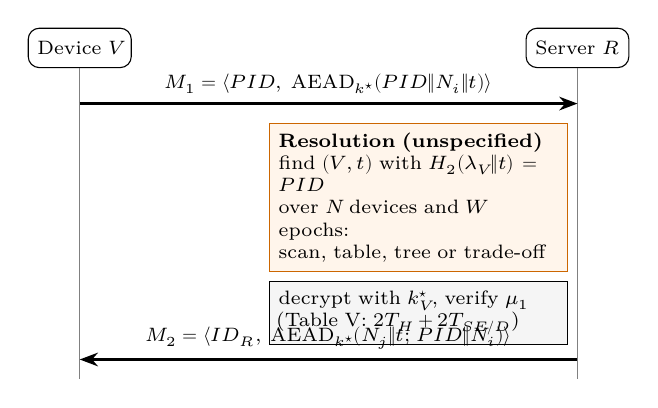
\begin{tikzpicture}[font=\scriptsize, >=Stealth, node distance=4mm]
\node[draw, rounded corners, minimum width=1.3cm, minimum height=5mm] (D) {Device $V$};
\node[draw, rounded corners, minimum width=1.3cm, minimum height=5mm, right=5.0cm of D] (S) {Server $R$};
\draw[gray] (D.south) -- ++(0,-3.95);
\draw[gray] (S.south) -- ++(0,-3.95);
\draw[->, thick] ($(D.south)+(0,-0.45)$) -- node[above, align=center]{$M_1=\langle PID,\;\mathrm{AEAD}_{k^\star}(PID\|N_i\|t)\rangle$} ($(S.south)+(0,-0.45)$);
\node[draw=orange!80!black, fill=orange!8, align=left, anchor=north east, text width=3.55cm] (R) at ($(S.south)+(-0.12,-0.7)$)
 {\textbf{Resolution (unspecified)}\\ find $(V,t)$ with $H_2(\lambda_V\|t)=PID$\\ over $N$ devices and $W$ epochs:\\ scan, table, tree or trade-off};
\node[draw, fill=gray!8, align=left, anchor=north east, text width=3.55cm] (V) at ($(R.south east)+(0,-0.12)$)
 {decrypt with $k^\star_V$, verify $\mu_1$\\ (Table V: $2T_H+2T_{SE/D}$)};
\draw[<-, thick] ($(D.south)+(0,-3.7)$) -- node[above]{$M_2=\langle ID_R,\;\mathrm{AEAD}_{k^\star}(N_j\|t;\,PID\|N_i)\rangle$} ($(S.south)+(0,-3.7)$);
\end{tikzpicture}
\caption{Where resolution sits. The server needs $k^\star_V$ to open $M_1$, but $V$ is hidden behind $PID$.}
\label{fig:flow}
\end{figure}

\section{Design Space}\label{sec:design}
We implemented seven strategies (Table~\ref{tab:design}). The first five keep the wire format of $M_1$. The last two need
a fresh $r$ in clear, so they change $M_1$. They are modelled at the resolution level, with the same keyed hash.
\begin{itemize}
\item \textbf{O1}, counter with a linear scan, is the behaviour of our original implementation. For each device it probes
epochs $\ell-L$ to $\ell+F$, where $\ell$ is the last accepted epoch, with $L=16$ and $F=8$ (window $W=25$).
\item \textbf{O2} keeps a table of every device's next $F$ pseudonyms and slides it after each acceptance.
\item \textbf{O3} and \textbf{O4} use clock epochs with a drift window $W_t=3$. O3 scans, and O4 extends a table once per
epoch.
\item \textbf{TM} is a rainbow table over $S=Nm$ points, with lifetime $m=128$ epochs per device, chain length
$\lceil S^{1/3}\rfloor$, $2S^{2/3}$ chains per table, and six tables.
\item \textbf{CR} and \textbf{MW} use $\delta=32$, so the tree has two levels up to $N=1024$.
\end{itemize}

\begin{table*}[t]
\centering
\caption{Design space. $N$: devices enrolled at the server; $L=16$, $F=8$, $W=L+F+1$; $W_t=3$; one table entry is 40\,B.
``Probes'' are expected $H_2$ evaluations per message, in steady state.}
\label{tab:design}
\footnotesize
\setlength{\tabcolsep}{3.2pt}
\begin{tabular}{@{}l l l l l l l l@{}}
\toprule
 & Epoch / $M_1$ & Probes, honest & Probes, forged & Precompute & Resolution state & Dropped $M_1$ & Linkability \\
\midrule
O1 & counter / unchanged & $\frac{(N-1)W}{2}+L+2$ & $NW$ & none & $8N$\,B & lockout after $F$ & none \\
O2 & counter / unchanged & $1$ (slide) & $0$ & $NF$ once & $(40F+8)N$\,B & lockout after $F$ & none \\
O3 & clock / unchanged & $\frac{(N-1)W_t}{2}+1$ & $NW_t$ & none & nonce cache & none & same epoch \\
O4 & clock / unchanged & $0$ & $0$ & $N$ per epoch & $40W_tN$\,B + cache & none & same epoch \\
TM & counter / unchanged & $\approx0.5$--$0.7\,S^{2/3}$ (meas.) & $\approx4\,S^{2/3}$ (meas.) & $\approx12S$ once & $\approx50\,S^{2/3}$\,B & none until $t=m$ & none \\
CR & none / $+r$ (128 b) & $\frac{N+1}{2}$ & $N$ & none & none & none & none \\
MW & none / $+r$, $+(d-1)$ tags & $\le\delta d$ & $\le\delta$ & none & $32\times$internal nodes & none & after compromise \\
\bottomrule
\end{tabular}
\end{table*}

\textbf{Validation.} For each strategy and each $N\in\{1,2,5,\dots,10^4\}$ (15 values), a script builds the server in
steady state. It resolves 200 pseudonyms of randomly drawn devices (50 for the scanning strategies above $N=2{,}000$) and 5 forged
ones, and counts
every $H_2$ call. For O1--O4 and CR, the forged and per-epoch counts and the state equal the closed forms exactly. O2
and O4 need exactly 1 and 0 probes per authentication. The honest means of O1, O3 and CR lie within four standard
errors of the formulas. MW never exceeds $\delta d$. In our parameter runs ($N=40$ to 500), the TM tables covered 99.6--99.8\% of
points, and in the sweep 9 of 2{,}100 honest pseudonyms were missed; the device then retries with its next epoch. Twelve unit tests run each wire-compatible
strategy through the full handshake. They check its probe counts, replay rejection and lockout behaviour, and they show
that two sessions in one clock epoch share a pseudonym. All 135 tests pass.

\section{Evaluation Method}\label{sec:method}
We follow the paper's evaluation conditions and change only the resolution term.
\begin{itemize}
\item \emph{Simulator and environment}: OMNeT++~\cite{omnet} 6.4 (Cmdenv), with Table~II of~\cite{base}: a
$1500\times1500$\,m area, 10\,Mbps, 500\,m range, 75.6\,mW, a 15\,$\mu$s quantum, servers at 5\% of the devices.
\item \emph{Protocol cost}: Tables~III--V of~\cite{base}. That is $2T_H+2T_{SE/D}=11.84$\,ms per side, 1{,}024 bits over
four messages, and $T_H=0.32$\,ms per probe.
\item \emph{Resolution cost}: for each server we look up the probes for its number of enrolled devices $n$ in the
measured cost model. It is exact for O1--O4 and CR, and interpolated between measured points for TM and MW. CR and MW
also add their extra $M_1$ bits.
\item \emph{Assumptions} (the paper does not fix these): an adversary share of 5\%, each sending forged $M_1$ at 1\,Hz; a
10\,s authentication window; each server enrols every device in its range; first-come-first-served server processing;
for O4, one epoch extension per server inside the window.
\item \emph{Runs}: five seeds per point and $N\in\{1,10,100,200,\dots,1000\}$, with and without adversaries. That is
960 runs in total, reported as means.
\end{itemize}
The model is ours, not the authors'. With the resolution term removed, it gives 23.86\,ms at $N=1$ and 24.07\,ms at
$N=1000$, against the paper's arithmetic value of 23.68\,ms. The difference is airtime and quantisation. The
\emph{base} column of Table~\ref{tab:ranked} ($N=1$) is therefore the paper's own figure: 23.68\,ms from Tables~III and~V,
and 320 bits of server storage from Table~VI. Storage at larger $N$ is Table~VI's 320 bits per enrolled device plus the
resolution state, averaged over the servers of the simulated network.

\section{Results}\label{sec:results}
\begin{table*}[t]
\centering
\caption{Strategies ranked from best to worst by mean session latency at $N=1000$ (5\% adversaries). Time: mean
per-session latency in the OMNeT++ model of the Table~II network, Table~III constants, mean of five seeds. Space: mean
storage per server. $N$ is the number of devices in the network; at $N\ge100$ each server enrols about a quarter of them. The base column ($N=1$) is the value published in~\cite{base}: 23.68\,ms (Tables~III, V) and 320 bits
(Table~VI).}
\label{tab:ranked}
\footnotesize
\setlength{\tabcolsep}{3pt}
\begin{tabular}{@{}c l l l l r r r r r r r r r r@{}}
\toprule
 & & & \multicolumn{2}{c}{Complexity per auth.} & \multicolumn{5}{c}{Mean session latency (ms)} & \multicolumn{5}{c}{Storage per server (KB)} \\
\cmidrule(lr){4-5}\cmidrule(lr){6-10}\cmidrule(l){11-15}
\# & & Strategy & Time & Space & base & 10 & 100 & 500 & 1000 & base & 10 & 100 & 500 & 1000 \\
\midrule
\rankedrows
\bottomrule
\end{tabular}
\end{table*}

\begin{figure*}[t]
\centering
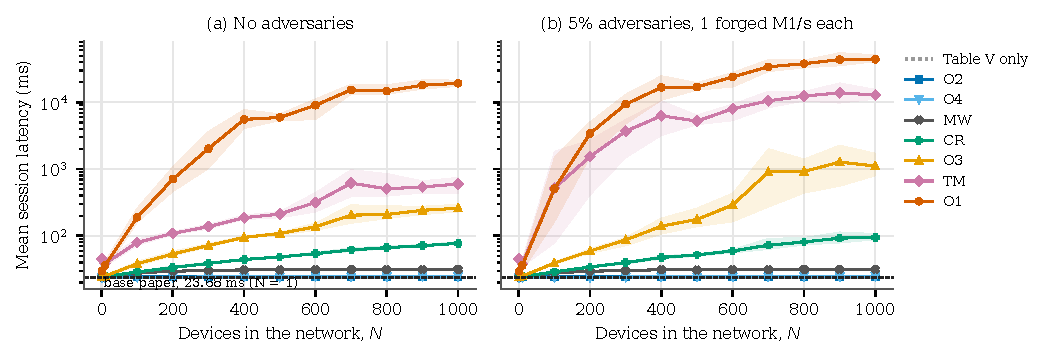
\includegraphics[width=0.92\textwidth]{figs/fig_latency.pdf}
\caption{Mean session latency against network size in the OMNeT++ model (log scale; band: minimum to maximum over five
seeds). Dotted: the paper's cost model with no resolution. Dashed: the paper's 23.68\,ms.}
\label{fig:latency}
\end{figure*}

\subsection{Ranking}
Table~\ref{tab:ranked} gives the ranking. The two table strategies, O2 and O4, stay within 1\,ms of the paper's figure up
to 1{,}000 devices. O2 needs one probe to slide the window, and O4 only the per-epoch extension. Their cost is memory: at
1{,}000 devices, about 93\,KB and 46\,KB per server, against 10\,KB for Table~VI alone. The key tree is third (31.4\,ms).
It changes $M_1$, and a compromised device leaks the internal keys it shares with others. The randomized hash lock (CR)
needs no extra state, but its latency grows linearly, to 95\,ms. The three scanning strategies with epochs saturate the
server: clock scan (O3) at 1.1\,s, the time-memory trade-off at 12.9\,s, and the counter scan (O1) at 44\,s. For O1 and
TM, the spread across seeds at $N=1000$ is 10.6\,s and 4.5\,s, because the latency depends on how many devices and
adversaries share the busiest server.

\subsection{Honest load against forged load}
Fig.~\ref{fig:latency} separates the two causes. Without adversaries (a), O1 already reaches 19.2\,s at 1{,}000 devices.
Each honest authentication costs about $12.5\,n$ probes, which is 1.0\,s of hashing at the $n\approx258$ devices that a
server enrols at $N=1000$ ($T_H=0.32$\,ms). Arrivals outpace this, so the server queue grows. The forged load (b) roughly doubles this, because every forged pseudonym costs a full miss scan of
$Wn$ probes. Such a pseudonym never resolves to a device, so the block-list, which counts failures per device, never sees
it. Fig.~\ref{fig:probes} shows the same effect for one server up to $10^4$ devices. A forgery costs O1 250{,}000 probes
and TM about 46{,}000, but costs O2 and O4 nothing, because a table miss needs no hash.

\begin{figure*}[t]
\centering
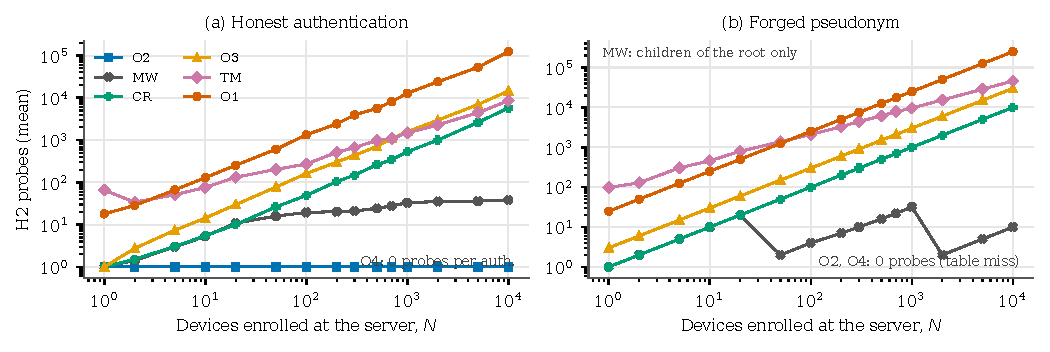
\includegraphics[width=0.92\textwidth]{figs/fig_probes.pdf}
\caption{Probes per message at one server, measured on the implementation (log-log). (a) Honest authentication. (b) A
forged, random pseudonym.}
\label{fig:probes}
\end{figure*}

\subsection{Time against memory}
Fig.~\ref{fig:storage} shows storage at one server, and each strategy's position in the time--memory plane at
$N=1000$. No strategy that keeps the wire format is both fast and small. O2 buys constant time with $F$ table entries per
device (328\,KB in total), and O4 with $W_t$ entries per device (144\,KB). TM sits in between, at 131\,KB and 1{,}478
probes. It is dominated here because its table must cover the device's whole lifetime ($m=128$ epochs), not just the
current window. MW is the only point that is both small and fast, and it pays with a different $M_1$ and a weaker
privacy model.

\begin{figure*}[t]
\centering
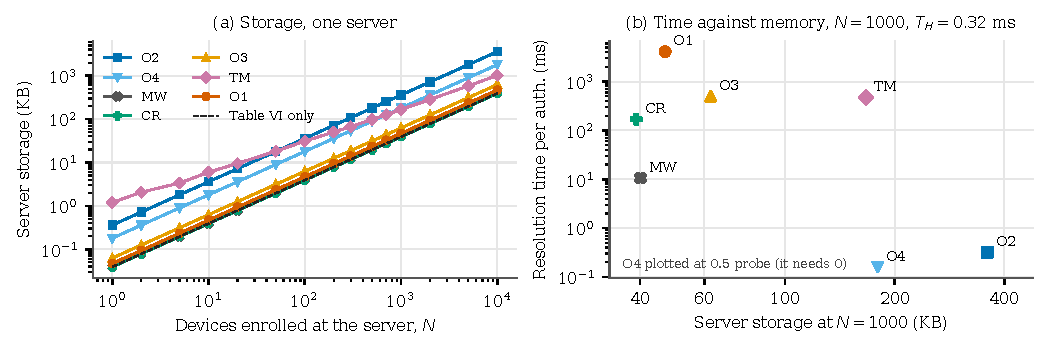
\includegraphics[width=0.92\textwidth]{figs/fig_storage.pdf}
\caption{(a) Server storage (Table~VI's 320 bits per device plus the resolution state) for one server. (b) Resolution
time per authentication ($T_H=0.32$\,ms per probe) against storage, at $N=1000$.}
\label{fig:storage}
\end{figure*}

\subsection{Desynchronisation}
With counter epochs, the device advances $t$ every time it builds $M_1$. The server searches at most $F$ epochs ahead of
the last one it accepted. In our implementation, an adversary who drops $F=8$ consecutive $M_1$ messages locks the device
out for good: every later handshake fails with an unknown pseudonym, with or without an earlier successful session. The
lockout holds for O1 and O2, and a unit test checks it for both. A device whose counter lives in RAM is also rejected as
a replay after a restart; we observed this for O1. Message dropping is within the threat model of~\cite{base}. Clock epochs (O3, O4), CR and MW have no
per-device counter, so they cannot desynchronise this way. TM tolerates any number of drops until $t$ reaches the
lifetime $m$.

\iffv
\section{Formal Verification}\label{sec:fv}
We modelled the exchange in ProVerif~2.05~\cite{proverif}, in the symbolic model with an active attacker
(Table~\ref{tab:fv}). Our hash, KDF and AEAD are free functions, and AEAD has associated data. The main model has
unbounded servers, unbounded honest and corrupt devices per server, and unbounded sessions. A corrupt device's $\lambda$
and $k^\star$ are given to the attacker. The server may resolve a pseudonym to \emph{any} enrolled device, and must then
decrypt and check $PID=H_2(\lambda_V\|t)$. So every result that holds, holds for every resolver that returns a correct
device. Epochs are fresh values, and the server keeps no replay state. Unlinkability is checked as observational
equivalence~\cite{blanchet08}, in the style of~\cite{arapinis}: one device running twice, against two devices running
once each. On both sides the server knows both devices and resolves with one destructor.

\begin{table}[t]
\centering
\caption{ProVerif results (all models finish in under 1\,s).}
\label{tab:fv}
\footnotesize
\begin{tabular}{@{}p{5.0cm}l@{}}
\toprule
Property & Result \\
\midrule
Q1/Q2 Session key secret (device / server side) & true \\
Q3 Server accepts $M_1$ of honest $V$ $\Rightarrow$ $V$ sent it & true \\
Q4 Same, injective (no replay state) & false (replay) \\
Q5 Device accepts $M_2$ $\Rightarrow$ server derived the same key, injective & true \\
FS Key secret after later leak of $k^\star$ & false \\
U1 Unlinkability, counter epochs & true \\
U2 Unlinkability, clock epochs, same epoch & fails (equal PIDs) \\
\bottomrule
\end{tabular}
\end{table}

These results separate the properties that the resolver cannot affect from those it decides:
\begin{itemize}
\item \emph{Independent of the resolver}: secrecy of the session key (Q1, Q2), agreement on $(V,R,N_i,t)$ (Q3), and
injective key agreement for the device (Q5). Q5 holds because $N_i$ is fresh and bound as associated data of $M_2$.
\item \emph{Decided by the epoch and replay choices}: injective authentication of the device (Q4) fails without replay
state. ProVerif finds a trace in which one $M_1$ is accepted twice. Injectivity therefore rests on the epoch window (O1,
O2, TM) or the nonce cache (O3, O4), which the specification leaves open. With clock epochs, the attacker links two
sessions in one epoch by testing their pseudonyms for equality (U2). With counter epochs, the equivalence holds (U1).
\item \emph{Forward secrecy}: it does not hold, and the base paper does not claim it. A later leak of $k^\star$ reveals
$N_i$, $N_j$ and $t$ from the ciphertexts, and with them the session key.
\end{itemize}
Q4 cannot be settled in ProVerif with the replay window included, because the window is mutable state. We check the
window by test instead, and leave a stateful proof (for example in Tamarin) to future work.
\fi

\section{Discussion}
\textbf{What a deployment should choose.} A server that uses counter epochs should precompute (O2). One probe per
authentication and no hashing on forged input remove both the scaling and the denial-of-service problem, at about
$40F$ bytes per device. The lockout after $F$ dropped messages remains, so the device needs a resynchronisation path, or
the server needs a larger $F$, which costs table space linearly. If devices have clocks, O4 has the lowest latency and
half the memory of O2. It makes sessions within one epoch linkable and needs a nonce cache for replay detection. The
epoch length then trades privacy against the per-epoch rebuild of $N$ probes. On-demand scanning (O1, O3) is
acceptable only for small $N$ and a trusted network. With 5\% adversaries, O1 is already 21 times the paper's
per-session cost at 100 devices.

\textbf{What the specification should state.} The protocol needs three decisions that it does not state: the epoch
semantics, the resolution method, and the replay state that makes device authentication injective. Its cost model
needs a resolution term. That term is $(N-1)W/2+L+2$ probes for an on-demand counter scan, and at least one probe or
one table lookup for a precomputed table. Its storage model needs the table.

\section{Limitations}
\begin{itemize}
\item The simulation is our model of the paper's stated environment, not the authors' simulation, which is not
available. The adversary rate, the authentication window and the enrolment rule are our assumptions, and the saturated
latencies of O1, O3 and TM depend on them.
\item We price probes with the paper's Table~III constant ($T_H=0.32$\,ms) and report no hardware timings.
\item CR and MW change $M_1$, and we model them at the resolution level only.
\item The TM parameters (six tables, $m=128$) are one point of its trade-off curve.
\item Our epoch, window and table choices are ours, not the paper's.
\item Conformance means agreement with our reading of Section~III, which only the authors can confirm.
\iffv
\item The ProVerif results are symbolic and assume perfect primitives.
\else
\item We give no formal proof.
\fi
\end{itemize}

\section{Conclusion}
A server cannot authenticate a device that it has not yet identified. In the protocol of~\cite{base}, that
identification is a required step with no specification and no cost in the model. Under the paper's own constants and
network, the choice of how to fill the gap decides whether the server stays at the paper's 23.68\,ms per session or
saturates at tens of seconds. It also decides whether a few dropped messages lock a device out, and whether forged
pseudonyms are free to send. Precomputed tables, the oldest answer from RFID private identification, keep the protocol's
cost claim intact at a memory cost of tens of kilobytes per server.
\iffv
The formal analysis shows that the protocol's secrecy and agreement properties do not depend on this choice, while
unlinkability and injective authentication do.
\fi
The implementation, the counting scripts, the OMNeT++ model\iffv, the ProVerif models\fi{} and all results are open at
\url{https://github.com/jaykerkar0405/hybrid-ecc-iot-auth}.

\balance
\begin{thebibliography}{99}
\bibitem{base} A. Al-Rasheed, R. Khan, A. Ahmad, A. Saeed, F. Alturise and S. Alkhalaf, ``A low-cost hybrid elliptic curve cryptography authentication protocol for trustworthy Internet of Things communication,'' \emph{IEEE Trans. Consum. Electron.}, vol.~72, no.~2, pp.~4483--4491, May 2026, doi:10.1109/TCE.2026.3662053.
\bibitem{weis} S. A. Weis, S. E. Sarma, R. L. Rivest and D. W. Engels, ``Security and privacy aspects of low-cost radio frequency identification systems,'' in \emph{Security in Pervasive Computing (SPC 2003)}, LNCS 2802. Springer, 2004, pp.~201--212.
\bibitem{ohkubo} M. Ohkubo, K. Suzuki and S. Kinoshita, ``Cryptographic approach to `privacy-friendly' tags,'' in \emph{RFID Privacy Workshop}, MIT, Cambridge, MA, USA, Nov. 2003.
\bibitem{molnar} D. Molnar and D. Wagner, ``Privacy and security in library RFID: Issues, practices, and architectures,'' in \emph{Proc. 11th ACM Conf. Computer and Communications Security (CCS)}, 2004, pp.~210--219.
\bibitem{avoine05} G. Avoine and P. Oechslin, ``A scalable and provably secure hash-based RFID protocol,'' in \emph{Proc. 3rd IEEE Int. Conf. Pervasive Computing and Communications Workshops (PerCom Workshops)}, 2005, pp.~110--114.
\bibitem{ado05} G. Avoine, E. Dysli and P. Oechslin, ``Reducing time complexity in RFID systems,'' in \emph{Selected Areas in Cryptography (SAC 2005)}, LNCS 3897. Springer, 2006, pp.~291--306.
\bibitem{tsudik} G. Tsudik, ``YA-TRAP: Yet another trivial RFID authentication protocol,'' in \emph{Proc. 4th IEEE Int. Conf. Pervasive Computing and Communications Workshops (PerCom Workshops)}, 2006, pp.~640--643.
\bibitem{hellman} M. E. Hellman, ``A cryptanalytic time-memory trade-off,'' \emph{IEEE Trans. Inf. Theory}, vol.~26, no.~4, pp.~401--406, 1980.
\bibitem{oechslin} P. Oechslin, ``Making a faster cryptanalytic time-memory trade-off,'' in \emph{Advances in Cryptology -- CRYPTO 2003}, LNCS 2729. Springer, 2003, pp.~617--630.
\bibitem{omnet} A. Varga and R. Hornig, ``An overview of the OMNeT++ simulation environment,'' in \emph{Proc. SIMUTools}, 2008.
\bibitem{hkdf} H. Krawczyk and P. Eronen, ``HMAC-based extract-and-expand key derivation function (HKDF),'' RFC 5869, 2010.
\bibitem{fips180} National Institute of Standards and Technology, ``Secure hash standard (SHS),'' FIPS PUB 180-4, 2015.
\bibitem{gcm} M. Dworkin, ``Recommendation for block cipher modes of operation: Galois/Counter Mode (GCM),'' NIST SP 800-38D, 2007.
\iffv
\bibitem{proverif} B. Blanchet, ``Modeling and verifying security protocols with the applied pi calculus and ProVerif,'' \emph{Foundations and Trends in Privacy and Security}, vol.~1, no.~1--2, pp.~1--135, 2016.
\bibitem{blanchet08} B. Blanchet, M. Abadi and C. Fournet, ``Automated verification of selected equivalences for security protocols,'' \emph{J. Log. Algebr. Program.}, vol.~75, no.~1, pp.~3--51, 2008.
\bibitem{arapinis} M. Arapinis, T. Chothia, E. Ritter and M. Ryan, ``Analysing unlinkability and anonymity using the applied pi calculus,'' in \emph{Proc. 23rd IEEE Computer Security Foundations Symp. (CSF)}, 2010, pp.~107--121.
\fi
\end{thebibliography}

\end{document}
